\label{Chapter1}

\section{Μεθοδολογία ανάπτυξης εφαρμογής}

\subsection{Διαθέσιμες μεθοδολογίες}

\subsubsection{Μοντέλο build and fix}

Το \textbf{μοντέλο build and fix} είναι ένα μοντέλο στο οποίο το λογισμικό έχει 
αναπτυχθεί χωρίς σχεδιασμό. Ουσιαστικά, κατασκευάζεται ένα αρχικό προϊόν και τροποποιείτε
μέχρι να ικανοποιήσει τον χρήστη. Το μοντέλο έχει δύο φάσεις:

\begin{itemize}
    \item Η φάση του \textbf{build}: Όπου ο κώδικας κατασκευάζεται
    και περνάει στην επόμενη φάση.
    \item Η φάση του \textbf{fix}: Όπου ο κώδικας έχει φτάσει σε bug και 
    error free στάδιο και μπορεί να παρουσιαστεί στον χρήστη και να τροποποιηθεί 
    κατάλληλα για να ικανοποιήσει τον τελικό χρήστη. 
\end{itemize}

\begin{center}
    \begin{tabular}{| p{8cm} | p{8cm} |}
        \hline
        \textbf{Πλεονεκτήματα} & \textbf{Μειονεκτήματα} \\
        \hline
        Χρειάζεται λιγότερη εμπειρία σε οποιονδήποτε άλλο τομέα εκτός του προγραμματισμού & Δεν υπάρχει ένας μετρητής στον οποίο κρίνετε ούτε η πρόοδος, ούτε η ποιότητα του προϊόντος και ούτε ο ρίσκο \\
        \hline
        Πολύ ταιριαστό για μικρά λογισμικά &  Ο κόστος είναι πελώριος επειδή χρειάζεται να γίνονται πάρα πολλές στο λογισμικό μέχρι να ικανοποιήσει τον τελικό χρήστη \\
        \hline
        Χρειάζεται λιγότερο πλάνο & Είναι πολύ ανεπίσημος τρόπος σχεδίασης ενός λογισμικού \\
        \hline
        & Η συντήρηση τέτοιων μοντέλων είναι δύσκολη \\
        \hline
    \end{tabular}
\end{center}

\subsubsection{Μοντέλο καταρράκτη}

\begin{figure}[th]
    \centering
    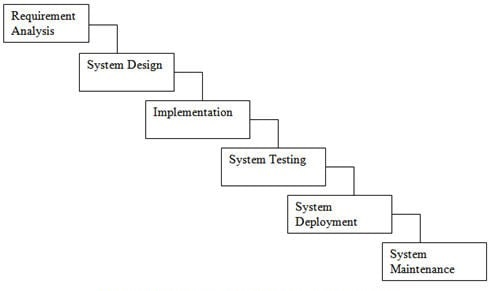
\includegraphics{Figures/waterfall.jpg}
    % \decoRule
    \caption[Το μοντέλο του καταρράκτη]{Το μοντέλο του καταρράκτη}
    \label{fig:waterfall}
\end{figure}
Το \textbf{μοντέλο του καταρράκτη (waterfall model)} είναι ένα από τα πιο κλασσικά παραδείγματα του life cycle. Η ανάπτυξη του λογισμικού είναι γραμμική και πάει από βήμα σε βήμα, η οποία πηγαίνει από βήμα σε βήμα με την ίδια ακριβώς δουλεία, χωρίς να υπάρχει δυνατότητα να μπορεί να γυρίσει πίσω. Κάθε βήμα έχει ξεχωριστό στόχο.

\begin{center}
    \begin{tabular}{| p{7cm} | p{2cm} | p{6.5cm} |}
        \hline
        \multicolumn{3}{|c|}{\textbf{Τα βήματα του μοντέλου καταρράκτη}} \\
        \hline
        \textbf{Είσοδος στο βήμα} & \textbf{Βήμα} & \textbf{Έξοδος του Βήματος} \\
        \hline
        Οι απαιτήσεις του λογισμικού πραγματοποιείται μέσω επικοινωνίας & Ανάλυσης &  Οι προδιαγραφές του λογισμικού είναι ορισμένες \\
        \hline
        Οι προδιαγραφές του λογισμικού είναι ορισμένες & Σχεδίασης & Σχεδιασμός του εγγράφου προδιαγραφών \\
        \hline
        Σχεδιασμός του εγγράφου προδιαγραφών & Ανάπτυξη & Δημιουργία εκτέλεσης προϊόντος \\
        \hline
        Δημιουργία εκτέλεσης προϊόντος & Δοκιμή & Έτοιμο προϊόν \\
        \hline
        Έτοιμο προϊόν & Υλοποίηση & Παραδοτέο λογισμικό \\
        \hline
        Παραδοτέο λογισμικό & Συντήρησης & Αλλαγές στις προδιαγραφές \\
        \hline
    \end{tabular}
\end{center}

\begin{center}
    \begin{tabular}{| p{8cm} | p{8cm} |}
        \hline
        \textbf{Πλεονεκτήματα} & \textbf{Μειονεκτήματα} \\
        \hline
        Αρκετά απλό στην κατανόηση & Χρειάζεται να είναι οι προδιαγραφές έτοιμες πριν ξεκινήσει η ανάπτυξη \\
        \hline
        Κάθε βήμα της ανάπτυξης συνεχίζει διαδοχικά & Δεν μπορούν να γίνουν αλλαγές στις προδιαγραφές σε μεταγενέστερα βήματα του μοντέλου. Αυτό σημαίνει ότι ένα λογισμικό μπορεί να μπει στο στάδιο της δοκιμής θα είναι πολύ δύσκολο να γίνουν οι απαραίτητες αλλαγές \\
        \hline
        Επιτρέπει ελέγχο στην δημιουργία ενός προγράμματος με προθεσμίες σε κάθε βήμα & Δεν υπάρχει καμία επικοινωνία με τον τελικό χρηστή όσο το λογισμικό αναπτύσσετε \\
        \hline
        Βοηθάει στον έλεγχο των χρονοπρογράμματων, των προϋπολογισμών  και του εγγράφου & Δεν παίρνει υπόψιν του τον ρίσκο της διοίκησης \\
        \hline
        & Θεωρεί ότι οι προδιαγραφές είναι σταθερές και δεν αλλάζουν κατά την διάρκεια του κύκλου ζωής  \\
        \hline
    \end{tabular}
\end{center}
